\begin{document}

\only<article>{
  \thispagestyle{empty}
  \pagecolor{white}\afterpage{\nopagecolor}
  \maketitle
}

\begin{frame}[plain]
 \titlepage
\end{frame}

\only<article>{
  \section*{Vorwort}
Die Gefahren, die im Internet herrschen, werden oft unterschätzt oder nicht wahrgenommen. Das Thema IT-Sicherheit wird im privaten Umfeld oft stiefmütterlich behandelt. Unter IT-Sicher\-heit versteht man alle Planungen, Maßnahmen und Kontrollen, die dem Schutz der IT dienen.
\vspace{12pt}

Dieses Dokument soll einen kurzen Überblick über die wichtigsten Bereiche der IT-Sicherheit geben.  Des Weiteren wird aufgezeigt, welche Möglichkeiten es gibt, wie man diese erkennen und man sich davor schützen kann. Diese Ratschläge betreffen sowohl den klassischen Com\-puter- als auch den Smartphone-Nutzer.
\vspace{12pt}

Der Abschnitt zur Datenschutzgrundverordnung (DVGVO) gibt einen sehr oberflächlichen Überblick über diese und kann nicht als rechtliche Beratung gesehen werden.
\vspace{12pt}

Die Präsentation wurde ursprünglich für die Laptop-Nutzer in der FF Steinheim e.V. konzipiert. Im Rahmen der firmeninternen Ausbildung der Auszubildenden Fachininformatiker wurde sie in einer früheren Version auch in der Firma \href{https://www.blackned.de}{blackned GmbH} gehalten. Die Feuerwehrversion wurde um einige Grundlagen und aktuelle Entwicklungen ergänzt.
\vspace{24pt}

Steinheim, \today \hfill Markus Flingelli
\newpage
}

\frame{
\only<presentation>{
  \frametitle{Inhaltsverzeichnis}
}
\tableofcontents[hideallsubsections]
}
\only<article>{
  \newpage
  \setcounter{page}{0}
  \pagenumbering{arabic}
}

\only<article>{
  \setlength\parindent{0pt}
}

\section{Einleitung}

\subsection{Definition}
\begin{frame}
\only<presentation>{
	\frametitle{Definition}
}
\begin{itemize}
	\item Unter IT-Sicherheit versteht man alle Planungen, Maßnahmen und Kontrollen, die dem Schutz der IT (Hardware und Software) dienen
	\item Klassische Ziele der IT-Sicherheit:
	\begin{itemize}
		\item Vertraulichkeit der Information
		\item Integrität der Informationen und Systeme
		\item Verfügbarkeit der Informationen und Systeme
	\end{itemize}
\end{itemize}
\end{frame}

\begin{frame}
\only<presentation>{
  \frametitle{BMI und BSI: Informationskampagne zur IT-Sicherheit}
}
\begin{figure}[ht]
	\centering
	\only<presentation>{
		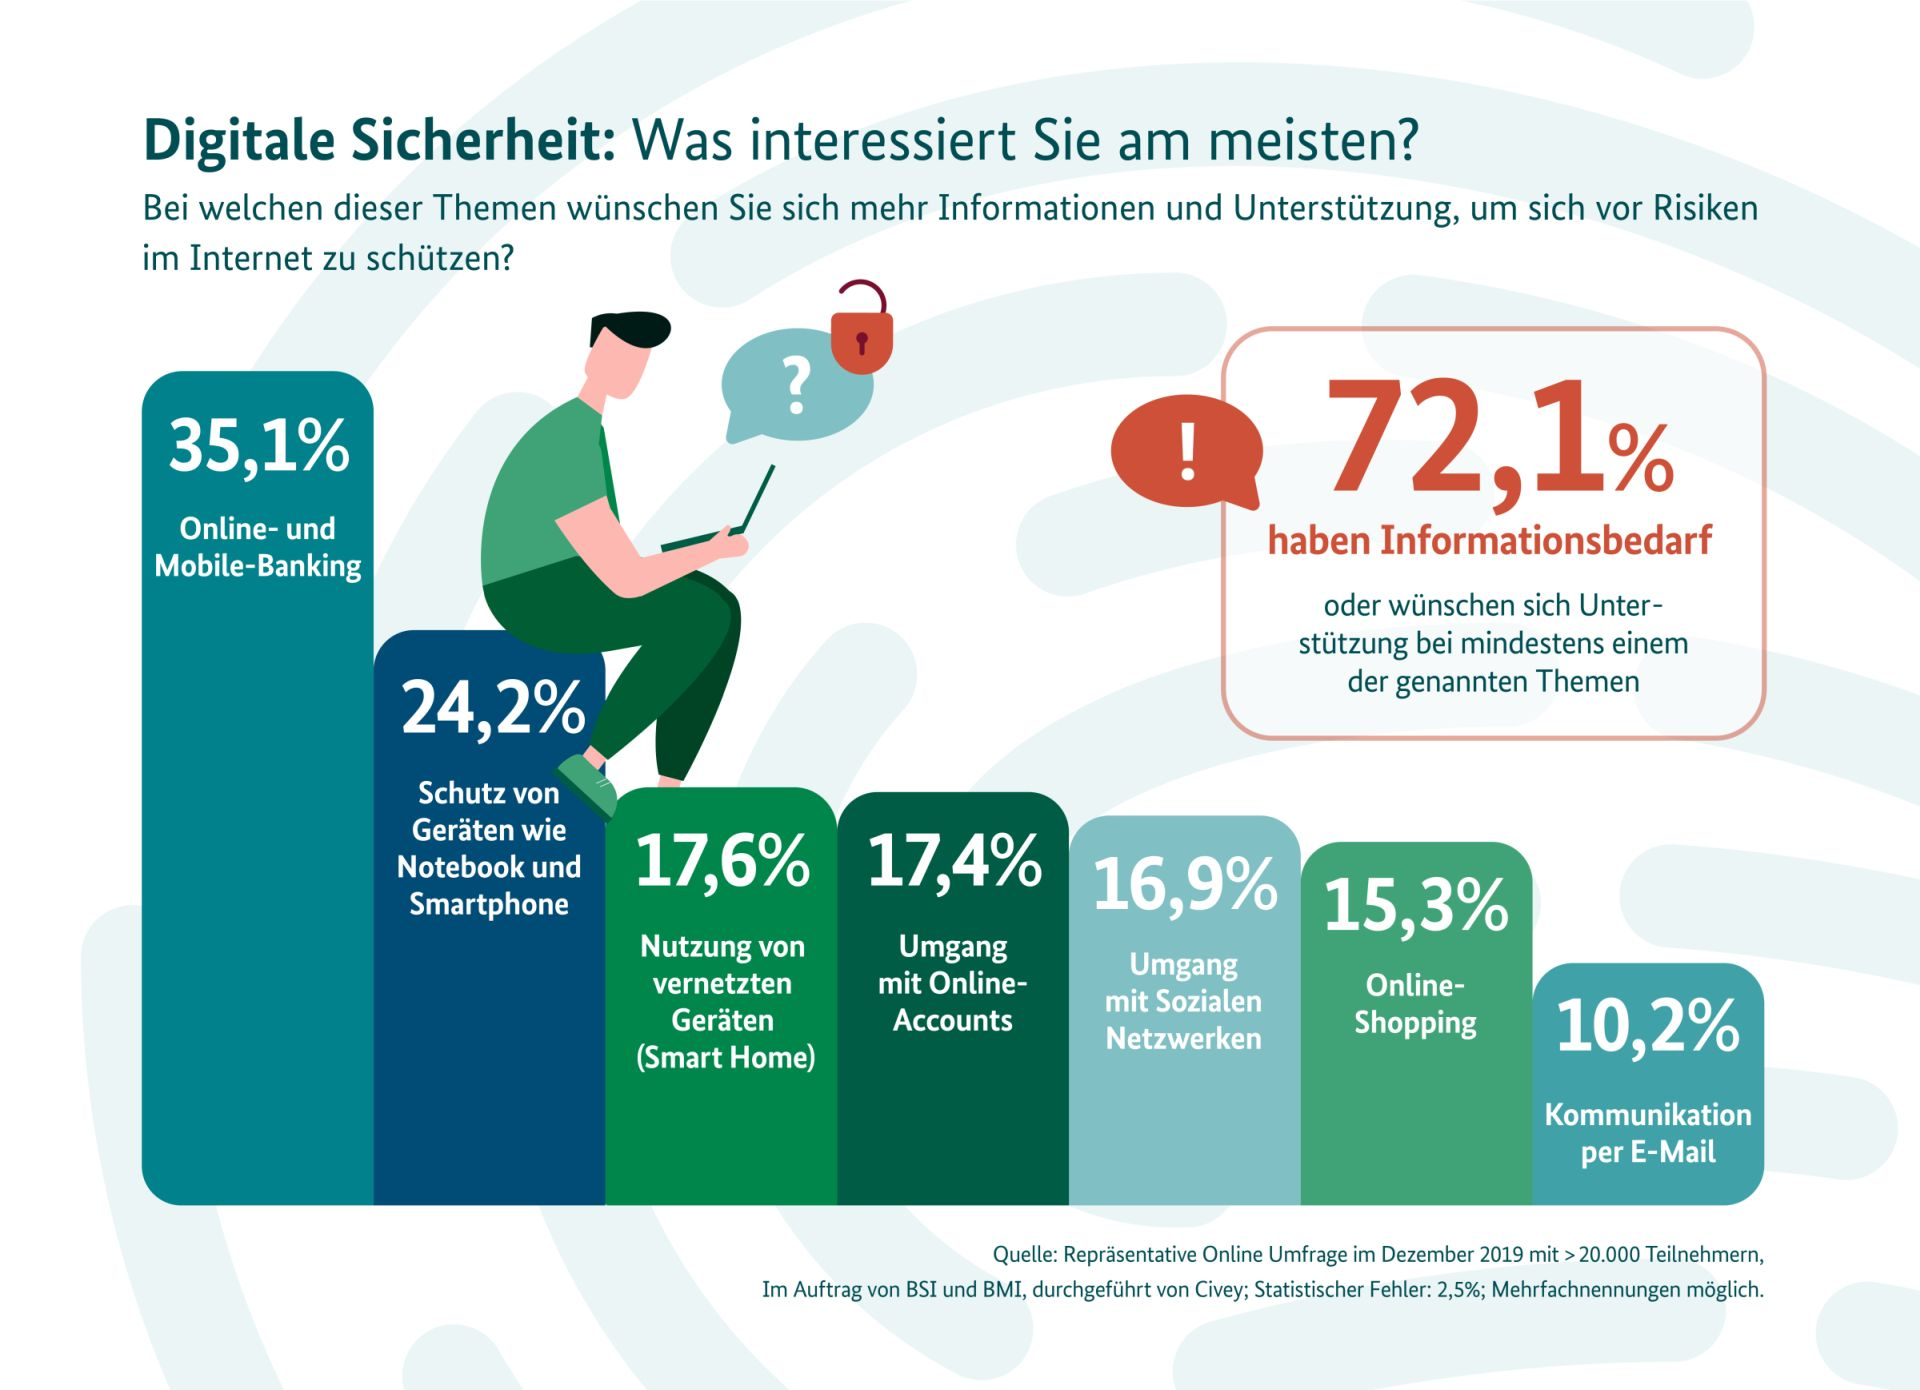
\includegraphics[width=.95\textwidth]{Umfrage-Safer-Internet-Day-200210.jpg}
	}
	\only<article>{
	  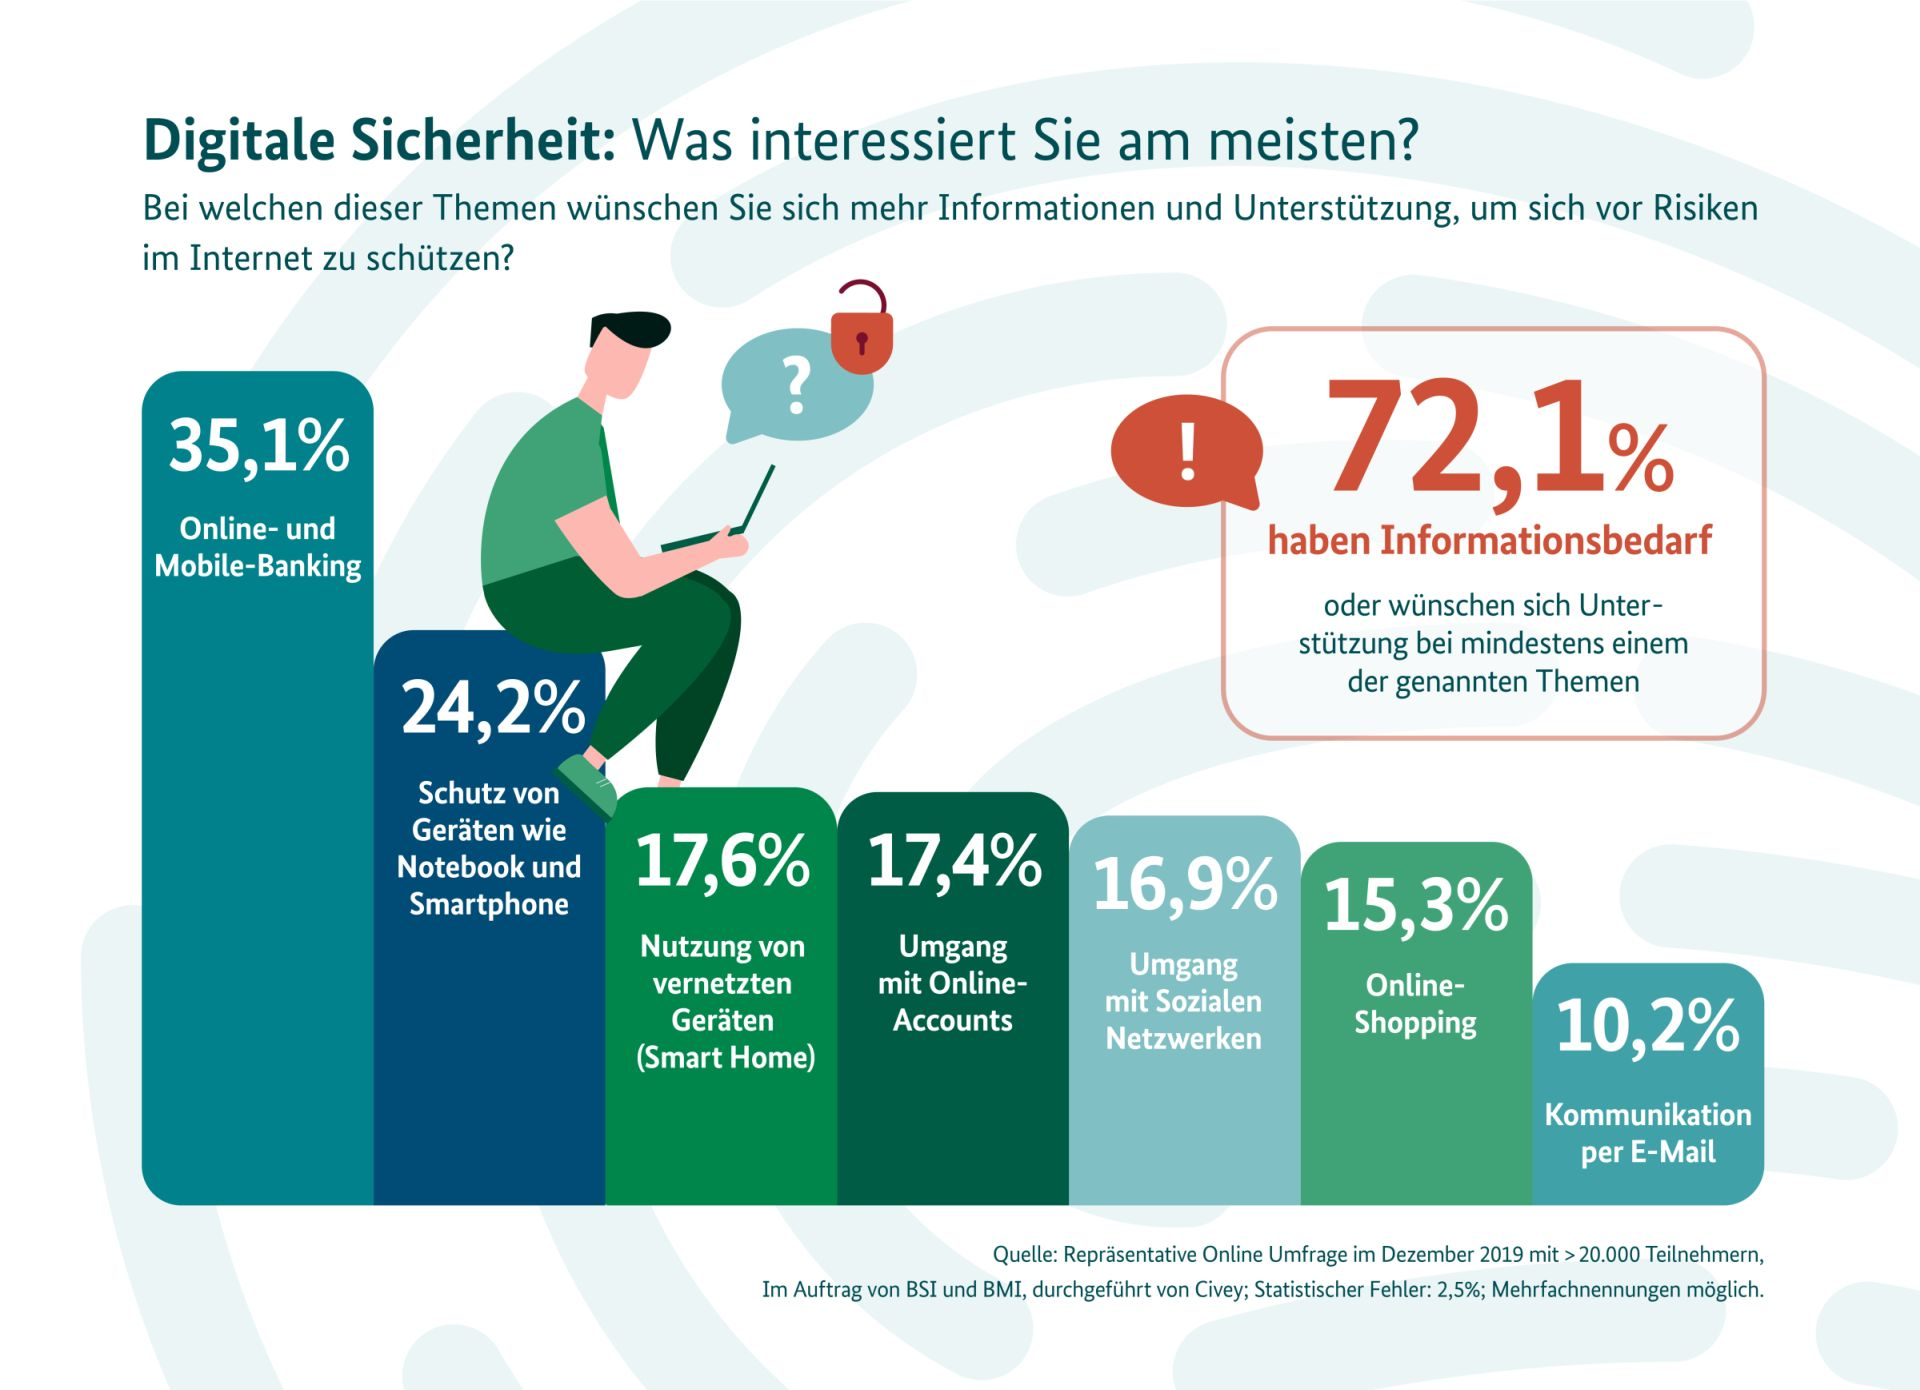
\includegraphics[width=.9\textwidth]{Umfrage-Safer-Internet-Day-200210.jpg}
	}
\end{figure}
\only<article>{
\scriptsize Quelle: \href{https://www.bsi.bund.de/DE/Presse/Pressemitteilungen/Presse2020/Safer-Internet-Day_100220.html}{https://www.bsi.bund.de/DE/Presse/Pressemitteilungen/Presse2020/Safer-Internet-Day\_100220.html}
\newline
\noindent\Hinweis[0.975\textwidth]{t}{Hinweise}{%
  \begin{itemize}
    \item Repräsentative Online-Umfrage des BMI und BSI mit 20.000 Teilnehmern
    \item Ergebnis: Mehr als 70 Prozent der Befragten wünschen sich mehr In\-form\-ation\-en über Ri\-si\-ken im Netz und eine größere Unterstützung im Bereich der digitalen Sicherheit
    \item Horst Seehofer:
    \begin{quote}
     \glqq Mit der Informationskampagne zur IT-Sicherheit wollen wir das Risikobewusstsein unserer Bürgerinnen und Bürger und ihre Fähigkeiten zur Problemlösung stärken, damit sie sich sicher im Netz bewegen. Die Umfrage zeigt, dass der Wunsch nach Unterstützung groß ist.\grqq
    \end{quote}
  \end{itemize}
}
}
\end{frame}

\section{Sicherheitshinweise}

\subsection{Allgemein}

\begin{frame}
\only<presentation>{
	\frametitle{Allgemein}
}
\begin{itemize}
	\item Beim Verlassen des Arbeitsplatzes ist Rechner zu sperren
	\item Bei der Bearbeitung von sensiblen Daten keinen unbefugten Personen auf den Bildschirm schauen lassen
	\item Nur Software aus vertrauenswürdigen Quellen verwenden
\end{itemize}
\end{frame}

\subsection{Kennwörter}

\only<presentation>{
	\begin{frame}
\frametitle{Kennwörter}
\begin{itemize}
  \item Alle Zeichenklassen verwenden (Groß-, Kleinbuchstaben, Zahlen, Sonderzeichen)
\item Lange Passwörter (> 15 Zeichen)
\item Für jeden Dienst bzw. Webseite ein eigenes Kennwort verwenden
\item Kennwörter nicht auf Zetteln oder Post-its am Monitor notieren
\item Kennwörter können im Passwortmanager (z.B. KeePass) gespeichert werden
\end{itemize}
\end{frame}

\begin{frame}
\frametitle{Kennwörter}
\begin{itemize}
  \item Kennwörter spätestens bei Verdacht auf Missbrauch ändern
\item Voreingestellte Kennwörter ändern
\item Kennwörter nicht an Dritte weitergeben und nicht per E-Mail versenden
\item Zwei-Faktor-Authentifizierung aktivieren
\item Kennwörter regelmäßig zu ändern, wird vom BSI nicht mehr explizit gefordert
\end{itemize}
\end{frame}
}
\only<article>{
	\begin{frame}
\begin{itemize}
  \item Alle Zeichenklassen verwenden (Groß-, Kleinbuchstaben, Zahlen, Sonderzeichen)
\item Lange Passwörter (> 15 Zeichen)
\item Für jeden Dienst bzw. Webseite ein eigenes Kennwort verwenden
\item Kennwörter nicht auf Zetteln oder Post-its am Monitor notieren
\item Kennwörter können im Passwortmanager (z.B. KeePass) gespeichert werden
  \item Kennwörter spätestens bei Verdacht auf Missbrauch ändern
\item Voreingestellte Kennwörter ändern
\item Kennwörter nicht an Dritte weitergeben und nicht per E-Mail versenden
\item Zwei-Faktor-Authentifizierung aktivieren
\item Kennwörter regelmäßig zu ändern, wird vom BSI nicht mehr explizit gefordert
  \only<article>{\item BSI-Video zu Kennwörtern: \href{http://multimedia.gsb.bund.de/BSI/Video/Sicher\_im\_Internet/Passwoerter.mp4}{\url{http://multimedia.gsb.bund.de/BSI/Video/Sicher\_im\_Internet/Passwoerter.mp4}}}
\end{itemize}
\end{frame}
}

\only<presentation>{
\begin{frame}
\frametitle{Kennwörter -- BSI-Video}
BSI-Video zu Kennwörtern:
\ifthenelse{\boolean{publicEdition}}{\newline \href{http://multimedia.gsb.bund.de/BSI/Video/Sicher\_im\_Internet/Passwoerter.mp4}{\url{http://multimedia.gsb.bund.de/BSI/Video/Sicher\_im\_Internet/Passwoerter.mp4}}}{\href{run:./Videos/Passwoerter.mp4}{Passwoerter.mp4}}
\end{frame}
}

\only<article>{\subsubsection{Beliebteste Kennwörter}}
\begin{frame}
\only<presentation>{
	\frametitle{Beliebteste Kennwörter}
}
\begin{longtable}{|r|r|r|}
\hline
\rowcolor{ffLightRed} & \textcolor{white}{Passwort} & \textcolor{white}{Häufigkeit} \\
\hline
 1 & \texttt{123456}    & 8,10 \permille \\\hline
 2 & \texttt{123456789} & 3,89 \permille \\\hline
 3 & \texttt{password}  & 1,89 \permille \\\hline
 4 & \texttt{qwerty}    & 1,85 \permille \\\hline
 5 & \texttt{12345}     & 1,38 \permille \\\hline
 6 & \texttt{12345678}  & 1,17 \permille \\\hline
 7 & \texttt{111111}    & 1,17 \permille \\\hline
 8 & \texttt{qwerty123} & 1,02 \permille \\\hline
 9 & \texttt{1q2w3e}    & 0,97 \permille \\\hline
10 & \texttt{123123}    & 0,85 \permille \\\hline
\end{longtable}
\scriptsize Quelle: \href{https://sec.hpi.de/ilc/statistics}{https://sec.hpi.de/ilc/statistics}, Stand 15.02.2020
\end{frame}

\only<article>{\subsubsection{Brute-Force-Attacke}}
\begin{frame}
\only<presentation>{
	\frametitle{Brute-Force-Attacke}
}
\begin{itemize}
  \item Bei einer Brute-Force-Attacke versucht ein Angreifer durch wiederholte und systematische Eingabe verschiedener Nutzernamen und Passwörter Login-Daten zu \glqq erraten\grqq.
  \item Umsetzung erfolgt meist über automatisierte Anwendungen auf Ressourcen-intensiver Rechnerinfrastruktur.
\end{itemize}
\end{frame}

\only<article>{\subsubsection{Benötigte Rechenzeit}}
\begin{frame}
\only<presentation>{
	\frametitle{Benötigte Rechenzeit}
}
\begin{center}
\begin{tikzpicture}\only<article>{[thick,scale=0.8, every node/.style={scale=0.8}]}
\foreach \x in {0,...,7}
  \draw [gray!50,dotted] (0,\x) -- (10,\x);
\draw[fill=ffUltraLightRed] (0.5cm,0cm) rectangle (1.5cm,.1cm) node at (1cm,.4cm) {1 Sekunde};   
\node at (1cm, -.5cm) {5};
\draw[fill=ffUltraLightRed] (2.5cm,0cm) rectangle (3.5cm,.3cm) node at (3cm,.7cm) {9 Sekunden};   
\node at (3cm, -.5cm) {7};
\draw[fill=ffUltraLightRed] (4.5cm,0cm) rectangle (5.5cm,.8cm) node at (5cm,1.1cm) {4,4 Tage};   
\node at (5cm, -.5cm) {9};
\draw[fill=ffUltraLightRed] (6.5cm,0cm) rectangle (7.5cm,1.6cm) node at (7cm,1.9cm) {7,6 Jahre};   
\node at (7cm, -.5cm) {11};
\draw[fill=ffUltraLightRed] (8.5cm,0cm) rectangle (9.5cm,6.8cm) node at (9cm,7.1cm) {359.000 Jahre};   
\node at (9cm, -.5cm) {13};
\node[rotate=90] at (-.5,3.5) {Ben\"otigte Zeit};
\node at (4,8) {\textbf{Ben\"otigte Rechenzeit bei 15 Millionen Schl\"usseln pro Sekunde}};
\end{tikzpicture}

\scriptsize Quelle: \href{https://www.cloudflare.com/learning/bots/brute-force-attack/}{https://www.cloudflare.com/learning/bots/brute-force-attack/}
\end{center}
\end{frame}

%\only<article>{
%\subsubsection{Zahlennamen}
%\begin{frame}
%\begin{longtable}{|r|l|}
%\hline
%\rowcolor{ffLightRed} 
%\textcolor{white}{Potenz} & \textcolor{white}{Zahlenname} \\
%\hline
%	$10^6$    & Million\\\hline
%	$10^9$    & Milliarde\\\hline
%	$10^{12}$ & Billion\\\hline
%	$10^{15}$ & Billiarde\\\hline
%	$10^{18}$ & Trillion\\\hline
%	$10^{21}$ & Trilliarde\\\hline
%	$10^{24}$ & Quadrillion\\\hline
%	$10^{27}$ & Quadrilliarde\\\hline
%	$10^{30}$ & Quintillion\\\hline
%\end{longtable}
%\end{frame}
%}


\subsection{Wechseldatenträger}

\begin{frame}
\only<presentation>{
	\frametitle{Wechseldatenträger}
}
\begin{itemize}
	\item Wechseldatenträger nur verwenden, wenn dessen Herkunft vertrauenswürdig ist
	\item Dateien mit vertraulichen Inhalten nur verschlüsselt ablegen (z.B. mit \href{http://www.7-zip.de/}{7-Zip} oder \href{https://www.veracrypt.fr}{VeraCrypt})
\end{itemize}
\end{frame}

\subsection{Datensicherung}

\begin{frame}
\only<presentation>{
	\frametitle{Datensicherung}
}
\begin{itemize}
	\item Regelmäßige Datensicherungen minimieren Ausfälle von Datenträgern oder Manipulationen an Datenbeständen
	\item Einspielen der Daten muss geübt werden
	\item Für Datensicherungsdatenträger gelten gleiche Sicherheitsvorgaben wie für das zu sichernde System
	\item Datensicherungen nicht im gleichen Raum oder Gebäude lagern
\end{itemize}
\end{frame}

\subsection{E-Mail}

\begin{frame}
\only<presentation>{
	\frametitle{E-Mail}
}
\begin{itemize}
	\item 3-Sekunden-Sicherheits-Check bei E-Mails
	\begin{enumerate}
		\item Ist der Absender bekannt?
		\item Ist der Betreff sinnvoll?
		\item Wird ein Anhang von diesem Absender erwartet?
	\end{enumerate}
	\item Spam-E-Mails direkt löschen
	\item Wenn möglich, E-Mails digital signieren und verschlüsseln
\end{itemize}
\end{frame}

\subsection{WLAN}

\begin{frame}
\only<presentation>{
	\frametitle{WLAN}
}
\begin{itemize}
	\item Nur sichere WLAN verwenden (WPA2\only<article>{\footnote{Wi-Fi Protected Access 2}})
	\item Verschlüsselung mit dem Standard WEP\only<article>{\footnote{Wired Equivalent Privacy}} ist unsicher und nicht zu empfehlen
	\item Netzwerknamen (SSID\only<article>{\footnote{Service Set Identifier}}) zufällig wählen (kein Rückschluss auf Betreiber oder verwendetes Gerät)
	\item Voreingestellte Kennwörter ändern
	\item WPS\only<article>{\footnote{Wi-Fi Protected Setup}}-PIN Verfahren deaktivieren
	\item WLAN nur bei Gebrauch einschalten
	\only<article>{\item BSI-Video zum WLAN: \href{http://multimedia.gsb.bund.de/BSI/Video/Sicher_im_Internet/WLAN.mp4}{\url{http://multimedia.gsb.bund.de/BSI/Video/Sicher\_im\_Internet/WLAN.mp4}}}
\end{itemize}
\end{frame}

\only<presentation>{
\begin{frame}
\frametitle{WLAN -- BSI-Video}
BSI-Video zum WLAN:
\ifthenelse{\boolean{publicEdition}}{\newline \href{http://multimedia.gsb.bund.de/BSI/Video/Sicher_im_Internet/WLAN.mp4}{\url{http://multimedia.gsb.bund.de/BSI/Video/Sicher\_im\_Internet/WLAN.mp4}}}{\href{run:./Videos/WLAN.mp4}{WLAN.mp4}}
\end{frame}
}

\subsection{Smartphones}

\only<presentation>{
	\begin{frame}
\frametitle{Smartphones}
\begin{itemize}
  \item Betriebssystem und Anwendungen (Apps) regelmäßig aktualisieren
\item Codes und Passwörter sowohl für die Entsperrung des Geräts als auch zum Öffnen von Apps sollten aktiviert und genutzt werden
\item Apps nur aus vertrauenswürdigen Quellen wie offiziellen App-Stores installieren
\item Back-up-Plan für den Fall des Verlust oder Beschädigung des Smartphones anlegen
\item Bei Verkauf oder Entsorgung Datenspeicher unwiederbringlich löschen 
\end{itemize}
\end{frame}

\begin{frame}
\frametitle{Smartphones}
\begin{itemize}
  \item Schnittstellen wie WLAN oder Bluetooth nur bei Gebrauch aktivieren
\item Vorsicht bei Nutzung offener WLAN-Hotspots (Einsatz von VPN)
\item Gerät nicht aus Augen lassen und nicht aus der Hand geben
\item Unbekannte Rufnummern nicht zurückrufen, insbesondere bei den Vorwahlen \textbf{0190} und \textbf{0180}
\item Vertrauliche Gespräche verschlüsseln
\end{itemize}
\end{frame}
}
\only<article>{
	\begin{frame}
\begin{itemize}
  \item Betriebssystem und Anwendungen (Apps) regelmäßig aktualisieren
\item Codes und Passwörter sowohl für die Entsperrung des Geräts als auch zum Öffnen von Apps sollten aktiviert und genutzt werden
\item Apps nur aus vertrauenswürdigen Quellen wie offiziellen App-Stores installieren
\item Back-up-Plan für den Fall des Verlust oder Beschädigung des Smartphones anlegen
\item Bei Verkauf oder Entsorgung Datenspeicher unwiederbringlich löschen 
  \item Schnittstellen wie WLAN oder Bluetooth nur bei Gebrauch aktivieren
\item Vorsicht bei Nutzung offener WLAN-Hotspots (Einsatz von VPN)
\item Gerät nicht aus Augen lassen und nicht aus der Hand geben
\item Unbekannte Rufnummern nicht zurückrufen, insbesondere bei den Vorwahlen \textbf{0190} und \textbf{0180}
\item Vertrauliche Gespräche verschlüsseln
\end{itemize}
\end{frame}
}

\subsection{Sicherer Umgang mit sozialen Netzwerken}

\only<presentation>{
	\begin{frame}
\frametitle{Sicherer Umgang mit sozialen Netzwerken}
\begin{itemize}
  \item Seien Sie zurückhaltend mit der Preisgabe persönlicher Informationen!
\item Erkundigen Sie sich über die Allgemeinen Geschäftsbedingungen und die Bestimmungen zum Datenschutz des genutzten sozialen Netzwerks!
\item Seien Sie wählerisch bei Kontaktanfragen -- Kriminelle \glqq sammeln\grqq\ Freunde, um Personen zu schaden!
\item Melden Sie \glqq Cyberstalker\grqq, die Sie unaufgefordert und dauerhaft über das soziale Netzwerk kontaktieren.
\end{itemize}
\end{frame}

\begin{frame}
\frametitle{Sicherer Umgang mit sozialen Netzwerken}
\begin{itemize}
  \item Verwenden Sie für jede Internetanwendung, insbesondere auch wenn Sie in verschiedenen sozialen Netzwerken angemeldet sind, ein unterschiedliches und sicheres Passwort!
\item Geben Sie keine vertraulichen Informationen über Ihren Arbeitgeber und Ihre Arbeit preis!
\item Prüfen Sie kritisch, welche Rechte Sie den Betreibern sozialer Netzwerke an den von Ihnen eingestellten Bildern, Texten und Informationen einräumen!
\item Wenn Sie \glqq zweifelhafte\grqq\ Anfragen von Bekannten erhalten, erkundigen Sie sich außerhalb sozialer Netzwerke nach der Vertrauenswürdigkeit dieser Nachricht!
\end{itemize}
\end{frame}

\begin{frame}
\frametitle{Sicherer Umgang mit sozialen Netzwerken}
\begin{itemize}
  \item Klicken Sie nicht wahllos auf Links -- Soziale Netzwerke werden verstärkt dazu genutzt, um Phishing zu betreiben!
\item Sprechen Sie mit Ihren Kindern über deren Aktivitäten in sozialen Netzwerken und klären Sie sie über die Gefahren auf!
\item Löschen eines Nutzerkontos: Erfahrungsgemäß findet sich die Möglichkeit zum Löschen eines Nutzerkontos erst nach längerem Suchen.
\end{itemize}
\end{frame}
}
\only<article>{
	\begin{frame}
\begin{itemize}
  \item Seien Sie zurückhaltend mit der Preisgabe persönlicher Informationen!
\item Erkundigen Sie sich über die Allgemeinen Geschäftsbedingungen und die Bestimmungen zum Datenschutz des genutzten sozialen Netzwerks!
\item Seien Sie wählerisch bei Kontaktanfragen -- Kriminelle \glqq sammeln\grqq\ Freunde, um Personen zu schaden!
\item Melden Sie \glqq Cyberstalker\grqq, die Sie unaufgefordert und dauerhaft über das soziale Netzwerk kontaktieren.
  \item Verwenden Sie für jede Internetanwendung, insbesondere auch wenn Sie in verschiedenen sozialen Netzwerken angemeldet sind, ein unterschiedliches und sicheres Passwort!
\item Geben Sie keine vertraulichen Informationen über Ihren Arbeitgeber und Ihre Arbeit preis!
\item Prüfen Sie kritisch, welche Rechte Sie den Betreibern sozialer Netzwerke an den von Ihnen eingestellten Bildern, Texten und Informationen einräumen!
\item Wenn Sie \glqq zweifelhafte\grqq\ Anfragen von Bekannten erhalten, erkundigen Sie sich außerhalb sozialer Netzwerke nach der Vertrauenswürdigkeit dieser Nachricht!
  \item Klicken Sie nicht wahllos auf Links -- Soziale Netzwerke werden verstärkt dazu genutzt, um Phishing zu betreiben!
\item Sprechen Sie mit Ihren Kindern über deren Aktivitäten in sozialen Netzwerken und klären Sie sie über die Gefahren auf!
\item Löschen eines Nutzerkontos: Erfahrungsgemäß findet sich die Möglichkeit zum Löschen eines Nutzerkontos erst nach längerem Suchen.
\end{itemize}
\end{frame}
}

\section{DSGVO}

\subsection{Allgemeines}
\begin{frame}
\only<presentation>{
	\frametitle{Allgemeines}
}
\begin{itemize}
	\item Nur notwendige Daten speichern (Datensparsamkeit)
	\item Bei Verarbeitung personenbezogener Daten muss angemessene Sicherheit gewährleistet werden
	\item Gesetzliche Speicherfristen sind zu beachten
	\item Auskunftsrecht des Betroffenen
	\item Informationsrecht bei Erhebung von Nutzerdaten
	\item Sicherheit der Verarbeitung
	\item IT-Sicherheitsvorgaben befolgen
\end{itemize}
\end{frame}

\subsection{Technische und organisatorische Maßnahmen}
\begin{frame}
\only<presentation>{
	\frametitle{Technische und organisatorische Maßnahmen}
}
\begin{itemize}
	\item Zustimmung zum Erfassen muss gegeben sein
	\item Einlegen von Widerspruch zur Datenerfassung muss gewährleistet sein
	\item Einsicht in erhobenen Daten muss möglich sein
	\item Verwendungszweck der Daten muss erfragt werden können
	\item Daten müssen sich berichtigen lassen können
	\item Daten müssen unter Umständen gesperrt werden können
\end{itemize}
\end{frame}

\only<article>{Bei Nichtbefolgen der DSGVO können hohe Bußgelder verhängt werden. Der Hamburgische Datenschutzbeauftragte hat wegen DSGVO-Verstößen ein Bußgeld in Höhe von 35.258.707,95 Euro gegen H\&M verhängt, weil die Firma in einem Servicecenter in Nürnberg Mitarbeiter massiv ausgespäht hatte. 

Es handelt sich um das höchste Bußgeld, das Aufsichtsbehörden hierzulande verhängten, seit die die Datenschutz-Grundverordnung (DSGVO) seit zweieinhalb Jahren anwendbar ist (siehe \href{https://www.heise.de/news/DSGVO-Deutsche-Rekordbusse-von-35-3-Millionen-Euro-gegen-H-M-4917437.html}{https://www.heise.de/news/DSGVO-Deutsche-Rekordbusse-von-35-3-Millionen-Euro-gegen-H-M-4917437.html}).}

\section{Spam}

\subsection{Grundbegriffe}

\begin{frame}
\only<presentation>{
	\frametitle{Grundbegriffe}
}
Spam bezeichnet den Massenversand nicht angeforderter Werbe-E-Mails und kann in folgende Bereiche unterteilt werden:
\begin{description}
	\item[Phising] Abfangen vertraulicher Daten wie Passwörter, Zugangsdaten oder Kreditkartennummern
	\item[Hoax] Falschmeldungen, die vergleichbar mit Zeitungsenten sind, im Internet kursieren
	\item[Scam] Scam-Mails enthalten Gewinnversprechen bzw. das Versprechen, schnell und mit einfachen Mitteln reich zu werden
\end{description}
\only<article>{Die Hälfte der E-Mails ist Spam und 99,99 \% davon werden mittlerweile automatisch blockiert.}
\end{frame}

\only<presentation>{
	\begin{frame}
\frametitle{Erkennen von Phising-E-Mails}
\begin{itemize}
  \item Die Absenderadressen sind zumeist gefälscht.
\item Die Anrede ist unpersönlich gehalten.
\item Dringender Handlungsbedarf wird signalisiert.
\item Drohungen kommen zum Einsatz.
\item Vertrauliche Daten (wie beispielsweise PINs und TANs) werden abgefragt, etwa in einem Formular innerhalb der E-Mail.
\item Die Mails enthalten Links oder Formulare, die vom Empfänger verfolgt beziehungsweise geöffnet werden sollen.
\end{itemize}
\end{frame}

\begin{frame}
\frametitle{Erkennen von Phising-E-Mails}
\begin{itemize}
  \item Die Nachrichten sind manchmal (aber nicht immer!) in schlechtem Deutsch verfasst. Die Gründe dafür: Sie werden manchmal von Computerprogrammen aus anderen Sprachen automatisch übersetzt.
\item Die E-Mails enthalten kyrillische Buchstaben oder falsch aufgelöste bzw. fehlende Umlaute (z.B. nur \glqq a\grqq\ statt \glqq ä\grqq\ beziehungsweise \glqq ae\grqq).
\end{itemize}
\end{frame}
}
\only<article>{
	\subsection{Erkennen von Phising-E-Mails}
	\begin{frame}
\begin{itemize}
  \item Die Absenderadressen sind zumeist gefälscht.
\item Die Anrede ist unpersönlich gehalten.
\item Dringender Handlungsbedarf wird signalisiert.
\item Drohungen kommen zum Einsatz.
\item Vertrauliche Daten (wie beispielsweise PINs und TANs) werden abgefragt, etwa in einem Formular innerhalb der E-Mail.
\item Die Mails enthalten Links oder Formulare, die vom Empfänger verfolgt beziehungsweise geöffnet werden sollen.
  \item Die Nachrichten sind manchmal (aber nicht immer!) in schlechtem Deutsch verfasst. Die Gründe dafür: Sie werden manchmal von Computerprogrammen aus anderen Sprachen automatisch übersetzt.
\item Die E-Mails enthalten kyrillische Buchstaben oder falsch aufgelöste bzw. fehlende Umlaute (z.B. nur \glqq a\grqq\ statt \glqq ä\grqq\ beziehungsweise \glqq ae\grqq).
  \item BSI-Video zu Phising: \href{http://multimedia.gsb.bund.de/BSI/Video/Sicher\_im\_Internet/Phishing.mp4}{\url{http://multimedia.gsb.bund.de/BSI/Video/Sicher\_im\_Internet/Phishing.mp4}}
\end{itemize}
\end{frame}
}

\only<presentation>{
\begin{frame}
\frametitle{Erkennen von Phising-E-Mails -- BSI-Video}
BSI-Video zu Phising:
\ifthenelse{\boolean{publicEdition}}{\newline  \href{http://multimedia.gsb.bund.de/BSI/Video/Sicher\_im\_Internet/Phishing.mp4}{\url{http://multimedia.gsb.bund.de/BSI/Video/Sicher\_im\_Internet/Phishing.mp4}}}{\href{run:./Videos/Phishing.mp4}{Phishing.mp4}}
\end{frame}
}


\subsection{Beispiele}

\only<article>{\subsubsection{Falsche Telekom-Rechnung}}

\begin{frame}
\only<presentation>{
  \frametitle{Falsche Telekom-Rechnung}
}
\only<article>{
  \begin{enumerate}
  \item[1] Absenderadresse entspricht nicht der Telekom
  \item[2] Seriöse Anbieter verschicken keine Rechnungen als Word-Dokumente (Gefahr von Viren)
  \item[3] Keine persönliche Anrede
  \item[4] Grammatikalischer Fehler
  \end{enumerate}
}
\begin{figure}[ht]
	\centering
	\only<presentation>{
		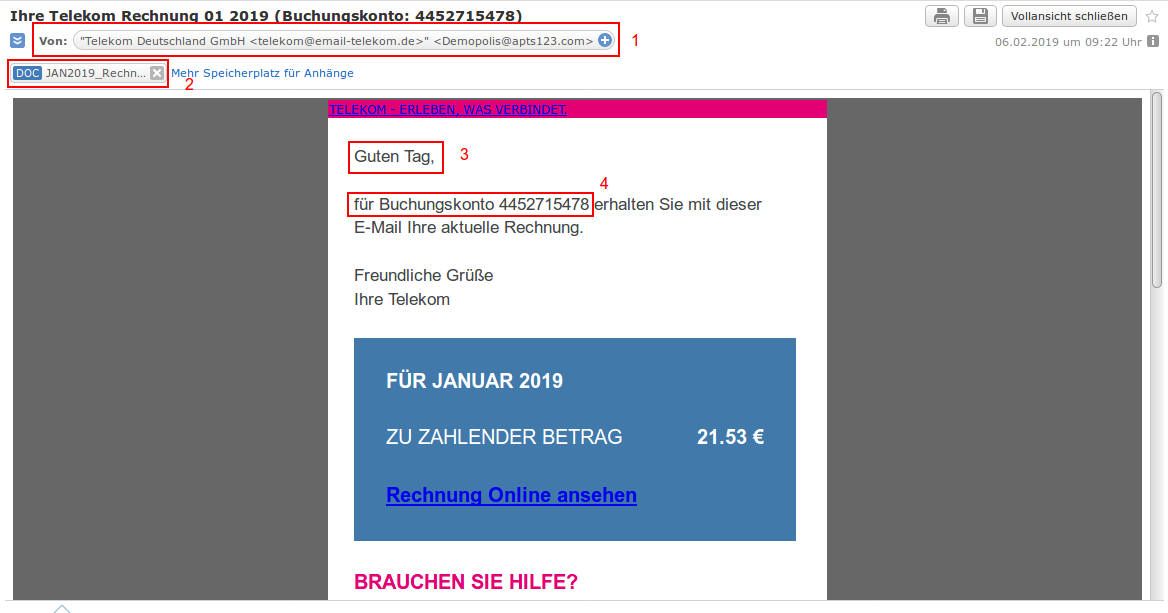
\includegraphics[width=.95\textwidth]{fake_telekom_rechnung_kommentar.png}
	}
	\only<article>{
	  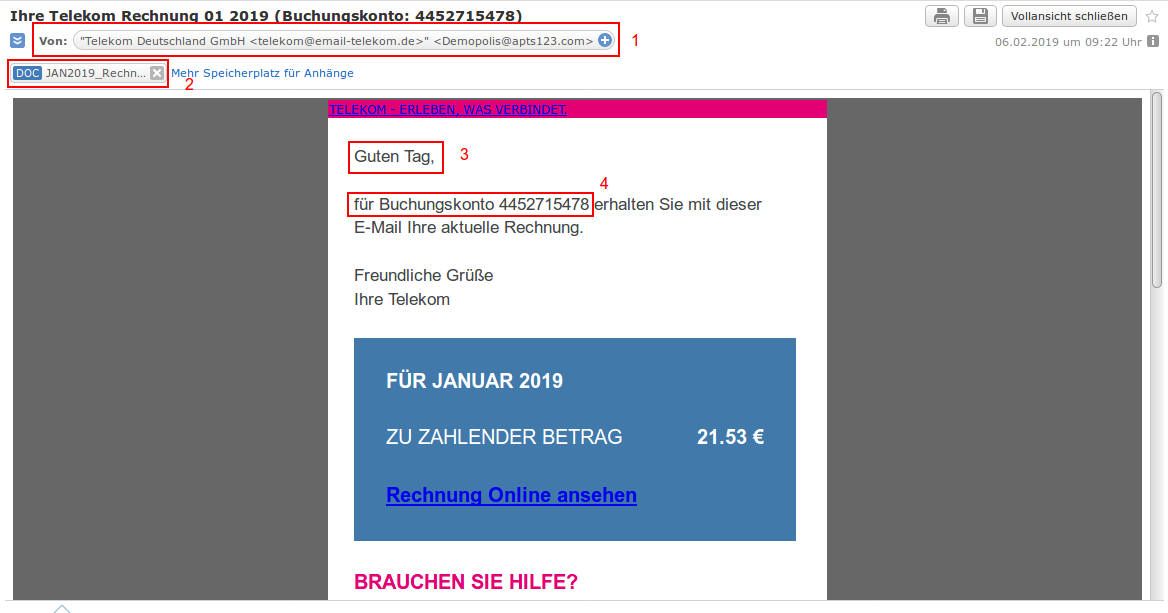
\includegraphics[width=.80\textwidth]{fake_telekom_rechnung_kommentar.png}
	}
\end{figure}
\end{frame}

\only<article>{\subsubsection{Vermeintliche E-Mail der Geschäftsleitung}}

\begin{frame}
\only<presentation>{
  \frametitle{Vermeintliche E-Mail der Geschäftsleitung}
}
\begin{itemize}
  \item Renommierter Großbetrieb im Memminger Norden wurde Opfer eines Betrugs
  \item Schadenssumme im sechsstelligen Bereich
  \item Finanzangestellte überwies wegen vermeintlicher E-Mail der Geschäftsleitung Betrag auf ausländisches Konto
  \item Falsche Identität des Absenders wurde erst einen Tag später bekannt, als Geldtransfer bereits abgeschlossen war
  \item Quelle: \href{https://www.new-facts.eu/memmingen-schadenstraechtiger-betrug-mittels-fingierter-e-mails-sechsstelliger-schadensbetrag-354520.html}{New Facts}, 25.01.2020
\end{itemize}
\end{frame}

\only<article>{\subsubsection{Online Banking}}

\begin{frame}
\only<presentation>{
  \frametitle{Online Banking}
}
\only<article>{
  \begin{enumerate}
  \item[1] Absenderadresse gehört offensichtlich zu Comdirect
  \item[2] E-Mail-Programm stuft E-Mail bereits als Junk ein
  \item[3] Fehlende persönliche Anrede
  \item[4] Rechtschreibfehler
  \item[5] Angegebener Link stimmt nicht mit tatsächlichem Link überein
  \end{enumerate}
}
\begin{figure}[ht]
	\centering
	\only<presentation>{
		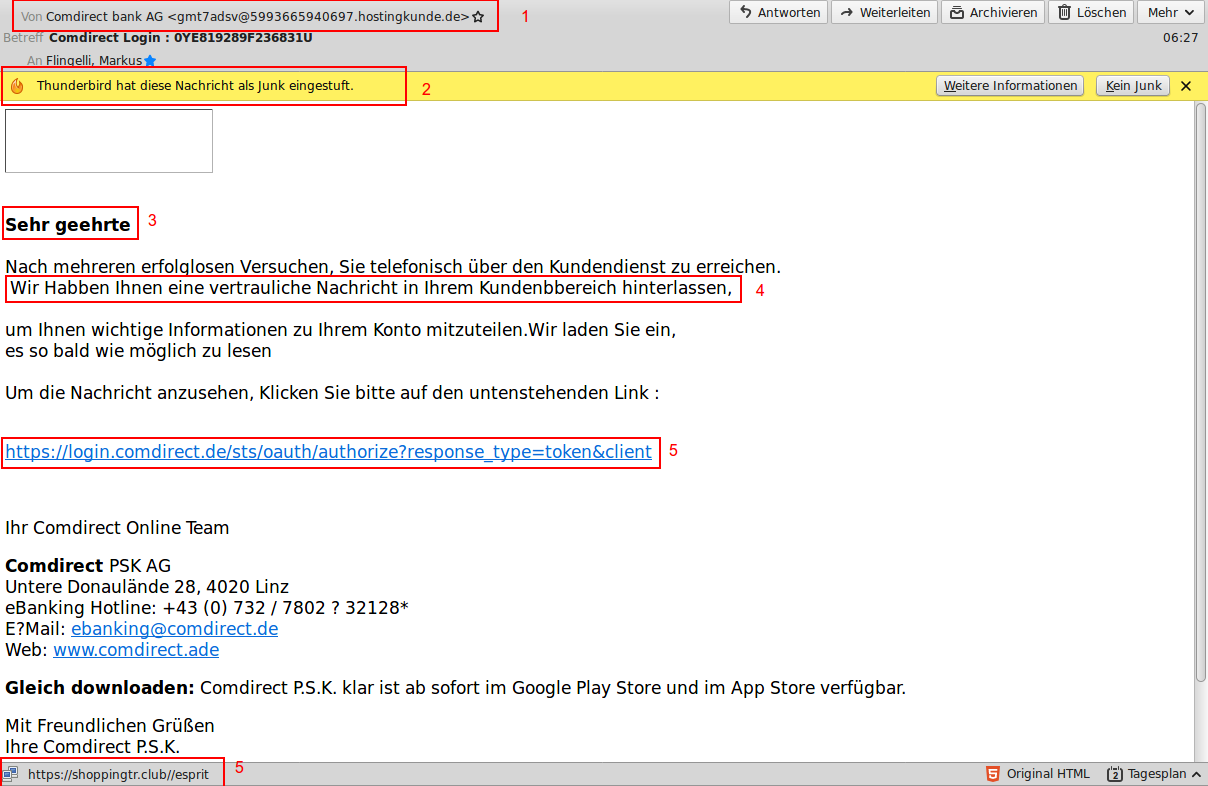
\includegraphics[width=.95\textwidth]{fake_online_banking.png}
	}
	\only<article>{
	  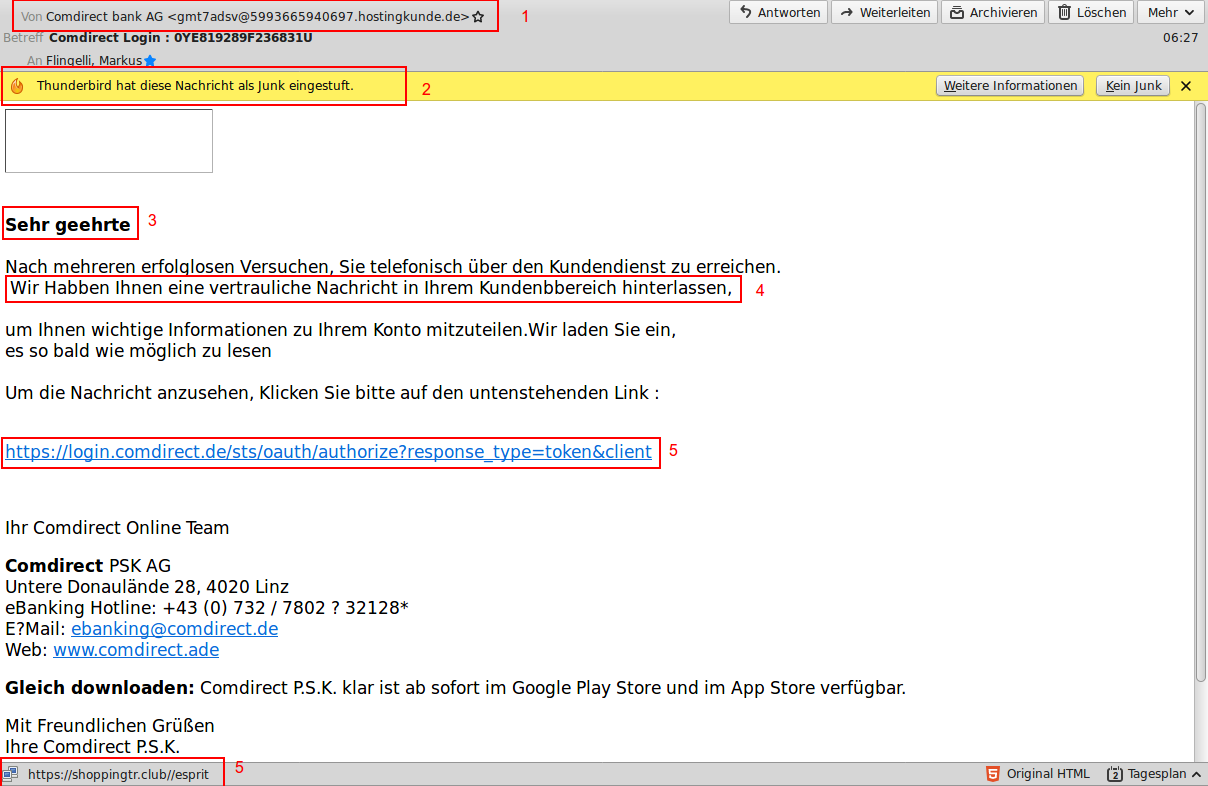
\includegraphics[width=.85\textwidth]{fake_online_banking.png}
	}
\end{figure}
\end{frame}

\only<article>{\subsubsection{Falscher Microsoft-Servicevertrag}}

\begin{frame}
\only<presentation>{
  \frametitle{Falscher Microsoft-Servicevertrag}
}
\only<article>{
  \begin{enumerate}
  \item[1] Absenderadresse gehört nicht zu Microsoft
  \item[2] Keine persönliche Begrüßung
  \end{enumerate}
}
\begin{figure}[ht]
	\centering
	\only<presentation>{
		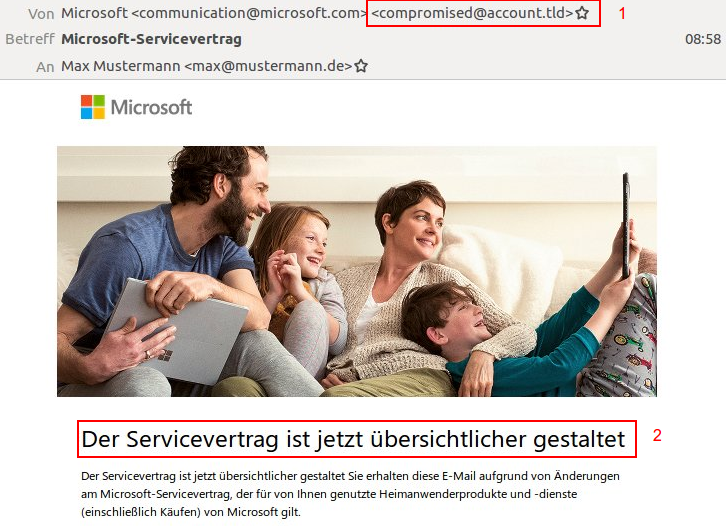
\includegraphics[width=.9\textwidth]{fake_microsoft_email.png}
	}
	\only<article>{
	  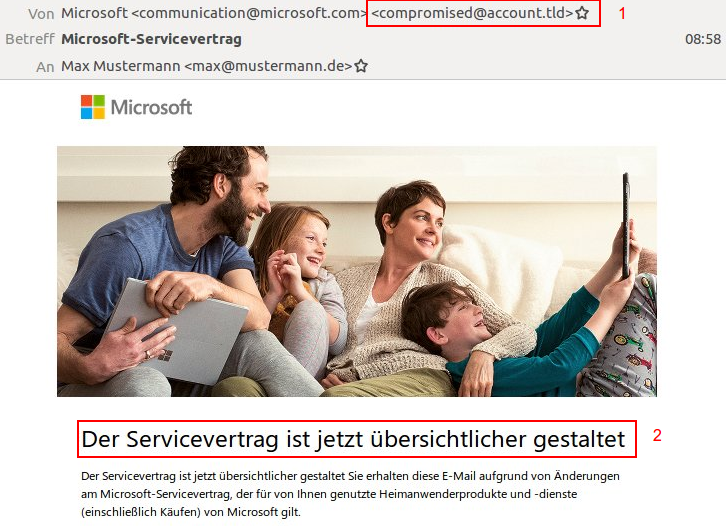
\includegraphics[width=.75\textwidth]{fake_microsoft_email.png}
	}
\end{figure}
\end{frame}

\only<article>{\subsubsection{Hoax}}

\begin{frame}
\only<presentation>{
	\frametitle{Hoax}
}
\begin{quotation}
Hi Leute,

ich wende mich an Euch, weil ich ziemlich verzweifelt bin. Ich hoffe, Ihr könnt mir und meiner Freundin helfen, und lest diesen Brief! Das Problem ist, dass meine Freundin an Leukämie erkrankt ist. Es hat sich herausgestellt, dass Sie nur noch wenige Wochen zu Leben hat. Aus diesem Grund seit Ihr meine letzte Chance Ihr zu helfen. 
[...]

Ich danke Euch für Eure Hilfe!!!

Gruß Toshiba65@aol.com
\end{quotation}
\end{frame}

\only<article>{\subsubsection{Scam}}

\begin{frame}
\only<presentation>{
	\frametitle{Scam}
}
\begin{figure}[ht]
	\centering
	\only<presentation>{
		
\includegraphics[width=.9\textwidth]{scam.png}
	}
	\only<article>{
	  
\includegraphics[width=.85\textwidth]{scam.png}
	}
\end{figure}
\end{frame}

\only<article>{\subsubsection{Schadsoftware}}
\begin{frame}
\only<presentation>{
	\frametitle{Schadsoftware}
}
Arten von  Schadsoftware (engl. Malware):
\begin{itemize}
	\item Viren und Würmer sind Programme, die sich von alleine verbreiten.
	\item Trojanische Pferde (oder auch Backdoors) führen auf einem Rechner eine verborgene Funktion aus; meistens um Daten auszuspionieren.
		\only<article>{
		\begin{itemize}
			\item Derzeit die zerstörerischste Schadsoftware laut US-CERT\footnote{CERT: Abkürzung für \glqq Computer Emergency Response Team\grqq}
			\item Nach Emotet-Angriff musste der Schweizer Fernsehhersteller Swiss Windows Konkurs anmelden und alle 170 Mitarbeiter entlassen.
			\item Quelle: \href{https://www.heise.de/security/meldung/FBI-Ransomware-Opfer-zahlten-ueber-140-Millionen-4675780.html}{https://www.heise.de/security/meldung/FBI-Ransomware-Opfer-zahlten-ueber-140-Millionen-4675780.html}
		\end{itemize}
		}
	\item Sparware forschen Computer und Nutzerverhalten aus.
	\item Scareware soll Nutzer verunsichern und dazu verleiten, schädliche Software zu installieren.
	\item Ransomware blockiert den Zugriff auf das Betriebssystem bzw. verschlüsselt potenziell wichtige Dateien und fordert den Benutzer zur Zahlung von Lösegeld auf
	\only<article>{
	\begin{itemize}
		\item Schaden durch Ransomware Crysis/Dhara laut FBI 61,24 Millionen US-Dollar (Quelle: \href{https://www.heise.de/security/meldung/FBI-Ransomware-Opfer-zahlten-ueber-140-Millionen-4675780.html}{https://www.heise.de/security/meldung/FBI-Ransomware-Opfer-zahlten-ueber-140-Millionen-4675780.html})
		\item Die erste Ransomware wurde im Jahr 1991 noch auf Diskette und per Post verschickt. Ein Biologe hat den Trojaner damals mit QuickBasic programmiert und in Umlauf gebracht. Betroffen waren AIDS-ForscherInnen, die ihre Daten nach Aktivierung des Datenträgers verschlüsselt vorfanden und aufgefordert wurden, die \glqq Jahreslizenz\grqq\ für die Benutzung ihres Rechners in Höhe von 189 Dollar zu erneuern -- zu zahlen per Verrechnungsscheck an ein Postfach in Panama.
	\end{itemize}
	}
\end{itemize}
\end{frame}

\only<article>{\subsection{Angriffe auf IT}}
\begin{frame}
\only<presentation>{
	\frametitle{Praxisreport 2020 Mittelstand -- IT-Sicherheit}
}
\begin{center}
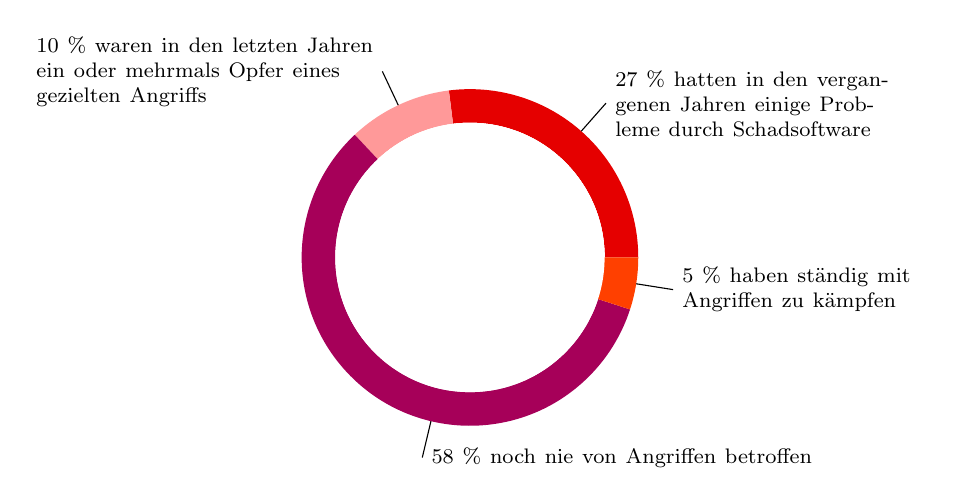
\begin{tikzpicture}[scale=0.95, every node/.style={scale=0.95}]
\foreach \anfang/\ende/\middle/\farbe/\anchor/\txtwidth/\description in {  
 	0/97.2/48.6/red!90!black/right/3.75cm/27 \% hatten in den vergangenen Jahren einige Probleme durch Schadsoftware, 
 	97.2/133.2/115.21/red!40!white/left/4.5cm/10 \% waren in den letzten Jahren ein oder mehrmals Opfer eines gezielten Angriffs, 
 	133.2/342/256.6/red!65!blue/right/5.5cm/58 \% noch nie von Angriffen betroffen,
 	342/360/351/red!50!orange/right/3.45cm/5 \% haben  st\"andig mit Angriffen zu k\"ampfen}
{ 	
  \draw[fill=\farbe,draw=none] (0,0) -- (\anfang:2.25cm) arc (\anfang:\ende:2.25cm);
  \draw[fill=white,draw=none] (0,0) circle (1.8cm);
  \draw (\middle:2.25cm) -- (\middle:2.75cm) node[rectangle, text width=\txtwidth,\anchor] {\baselineskip=8pt \footnotesize \description\par};
}
\end{tikzpicture}
\end{center}
\scriptsize Quelle: \href{https://www.sicher-im-netz.de/dsin-praxisreport-2020-mittelstand-it-sicherheit}{https://www.sicher-im-netz.de/dsin-praxisreport-2020-mittelstand-it-sicherheit}
\end{frame}

\only<article>{\subsection{Wirtschaftlicher Schaden}}

\begin{frame}
\only<presentation>{
  \frametitle{Wirtschaftlicher Schaden}
}
\begin{itemize}
  \item Schätzung der Firma Symantec für das Jahr 2017
  \item 978 Millionen Menschen in 20 Ländern von Cyberkriminalität betroffen
  \item Entschandener Schaden liegt bei etwa 172 Milliarden US Dollar
  \item Quelle: Bruce Schneier -- Click here to kill everybody, 1. Auflage 2019, mitp
\end{itemize}
\end{frame}

\section{Sicherheitsirrtümer}

\subsection{Internet-Sicherheit}

\only<presentation>{
	\begin{frame}
\frametitle{Internet-Sicherheit}
\begin{itemize}
  \item Sicherheitsvorkehrungen sind unnötig, die Hacker knacken doch sowieso alles.
\item Meine PC-Firewall schützt mich vor allen Angriffen aus dem Internet.
\item Wenn ich ein aktuelles Virenschutzprogramm habe, muss ich Updates für andere Software nicht sofort installieren.
\item Ein einziges langes Buchstaben- und Zeichen-Passwort reicht für meine Online-Dienste vollkommen aus.

\end{itemize}
\end{frame}

\begin{frame}
\frametitle{Internet-Sicherheit}
\begin{itemize}
  \item Ich surfe nur auf vertrauenswürdigen Seiten, darum muss ich mich nicht vor Cyber-Angriffen schützen.
\item Wenn der eigene Rechner infiziert ist, merkt man das.
\item Ich surfe nicht auf Pornoseiten, deshalb kann ich mir nichts einfangen.
\item Sehe ich das Schloss im Browser, ist alles in Ordnung.
\end{itemize}
\end{frame}
}
\only<article>{
	\begin{frame}
\begin{itemize}
  \item Sicherheitsvorkehrungen sind unnötig, die Hacker knacken doch sowieso alles.
\item Meine PC-Firewall schützt mich vor allen Angriffen aus dem Internet.
\item Wenn ich ein aktuelles Virenschutzprogramm habe, muss ich Updates für andere Software nicht sofort installieren.
\item Ein einziges langes Buchstaben- und Zeichen-Passwort reicht für meine Online-Dienste vollkommen aus.

  \item Ich surfe nur auf vertrauenswürdigen Seiten, darum muss ich mich nicht vor Cyber-Angriffen schützen.
\item Wenn der eigene Rechner infiziert ist, merkt man das.
\item Ich surfe nicht auf Pornoseiten, deshalb kann ich mir nichts einfangen.
\item Sehe ich das Schloss im Browser, ist alles in Ordnung.
\end{itemize}
\end{frame}
}


\subsection{Mobile Sicherheit}

\begin{frame}
\only<presentation>{
	\frametitle{Mobile Sicherheit}
}
\begin{itemize}
	\item Meine Daten sind in der Cloud sicher vor Fremdzugriff geschützt.
	\item Das Surfen in öffentlichen WLANs spart nicht nur Kosten, sondern ist auch sicher.
	\item Wenn ich mir ein neues Smartphone kaufe, habe ich automatisch ein sicheres Gerät.
	\item Ich habe natürlich automatische Updates und Aktualisierungen des Betriebssystems und von Apps aktiviert, daher muss ich mich um Schwachstellen nicht kümmern.
\end{itemize}
\end{frame}

\subsection{Computer-Sicherheit}

\only<presentation>{
	\begin{frame}
\frametitle{Computer-Sicherheit}
\begin{itemize}
  \item Wenn ich einen Virus oder ein anderes Schadprogramm auf dem Computer habe, macht sich dieser auch bemerkbar.
\item Ich habe nichts zu verbergen und keine wichtigen Daten, also bin ich doch kein Ziel für Cyber-Kriminelle und muss mich deshalb nicht schützen.
\item Meine Daten sind doch in der Cloud, darum brauche ich kein Back-up.

\end{itemize}
\end{frame}

\begin{frame}
\frametitle{Computer-Sicherheit}
\begin{itemize}
  \item Wenn ich alle Daten von meinem Gerät lösche und anschließend den Papierkorb leere, sind die Daten ein für alle mal weg.
\item Wenn ich ein gutes Kennwort habe, dann kann keiner meine E-Mails lesen.
\item Geheime Sicherheitsverfahren sind immer sicherer als öffentlich bekannte Verfahren.
\end{itemize}
\end{frame}
}
\only<article>{
\begin{frame}
\begin{itemize}
  \item Wenn ich einen Virus oder ein anderes Schadprogramm auf dem Computer habe, macht sich dieser auch bemerkbar.
\item Ich habe nichts zu verbergen und keine wichtigen Daten, also bin ich doch kein Ziel für Cyber-Kriminelle und muss mich deshalb nicht schützen.
\item Meine Daten sind doch in der Cloud, darum brauche ich kein Back-up.

  \item Wenn ich alle Daten von meinem Gerät lösche und anschließend den Papierkorb leere, sind die Daten ein für alle mal weg.
\item Wenn ich ein gutes Kennwort habe, dann kann keiner meine E-Mails lesen.
\item Geheime Sicherheitsverfahren sind immer sicherer als öffentlich bekannte Verfahren.
\end{itemize}
\end{frame}
}

\begin{frame}
\only<presentation>{
	\frametitle{Negativbeispiele}
}
\begin{itemize}
	\item \href{https://www.heise.de/ct/}{c't}-Leser findet auf bei eBay ersteigerten Rechner Zehntausende Bürgerdaten aus einer Kfz-Zulassungsstelle und dem Jugendamt der Stadt Coburg
	\item Süddeutsche Zeitung berichtet über einen Förster, der auf einem Gebraucht-Laptop der Bundeswehr Pläne für den Raketenwerfer \glqq Mars\grqq\ fand
	\item Mitarbeiter fanden auf gebrauchten Laptop für 90 Euro auf eBay der Bundeswehr Pläne für das Flugabwehrsystem \glqq Ozelot\grqq
	\item \scriptsize{Quelle: \href{https://www.heise.de/newsticker/meldung/Bundeswehr-Plaene-fuer-Flugabwehrsystem-auf-Gebrauchtrechner-von-eBay-4683375.html}{https://www.heise.de/newsticker/meldung/Bundeswehr-Plaene-fuer-Flugabwehrsystem-auf-Gebrauchtrechner-von-eBay-4683375.html}}
\end{itemize}
\end{frame}

\subsection{E-Mail}

\begin{frame}
\only<presentation>{
	\frametitle{E-Mail}
}
\begin{itemize}
	\item Wenn ich eine E-Mail nur anschaue, aber keinen Anhang öffne, kann nichts passieren.
	\item Das Antworten auf Spam-Mails birgt keine Gefahr, man kann auch den Links zum Löschen aus dem Verteiler folgen.
	\item Eine E-Mail kommt immer von der Adresse, die im Absenderfeld steht.
	\item Phishing-Mails sind leicht zu erkennen.
	\item Ich öffne nur Mails von Freunden und Bekannten, deshalb kann mir nichts passieren.
\end{itemize}
\end{frame}

\section{Mehrfachnutzung Computer}

\only<presentation>{
	\begin{frame}
\frametitle{Computer-Mehrfachnutzung}
\begin{itemize}
  \item Nicht mit Administratorenrechten arbeiten
\item Unterschiedliche Benutzerkonten einrichten
\item Immer aktuelle Software einsetzen
\item Nutzungsberechtigungen einschränken
\item Nutzungsmöglichkeiten für Kinder einschränken

\end{itemize}
\end{frame}

\begin{frame}
\frametitle{Computer-Mehrfachnutzung}
\begin{itemize}
  \item Sensible Daten auf separaten Geräten bearbeiten
\item Vorsichtig mit Passwörtern umgehen
\item Verlauf löschen und wenn möglich, Inkognito-Modus verwenden
\item Daten regelmäßig sichern
\end{itemize}
\end{frame}
}
\only<article>{
	\begin{frame}
\begin{itemize}
  \item Nicht mit Administratorenrechten arbeiten
\item Unterschiedliche Benutzerkonten einrichten
\item Immer aktuelle Software einsetzen
\item Nutzungsberechtigungen einschränken
\item Nutzungsmöglichkeiten für Kinder einschränken

  \item Sensible Daten auf separaten Geräten bearbeiten
\item Vorsichtig mit Passwörtern umgehen
\item Verlauf löschen und wenn möglich, Inkognito-Modus verwenden
\item Daten regelmäßig sichern
\end{itemize}
\end{frame}
}

\section{Hacking}

\begin{frame}
\only<presentation>{
  \frametitle{Abgreifen Zugangsdaten}
}
\begin{itemize}
	\item Anmeldung auf der Website \href{http://steinheim.ffw-mm.de/}{http://steinheim.ffw-mm.de/}
	\item Verwendeter Nutzername: \textbf{flingo}
	\item Verwendetes Kennwort: \textbf{MeinKennwortVerateichnicht}
\end{itemize}
\end{frame}

\begin{frame}
\only<presentation>{
  \frametitle{Abgreifen Zugangsdaten}
}
\only<article>{
	\newpage
	Das Abgreifen der Zugangsdaten ist möglich, da die Verbindung zur Webseite nicht abgesichert ist.
}
\begin{figure}[ht]
	\centering
	\only<presentation>{
		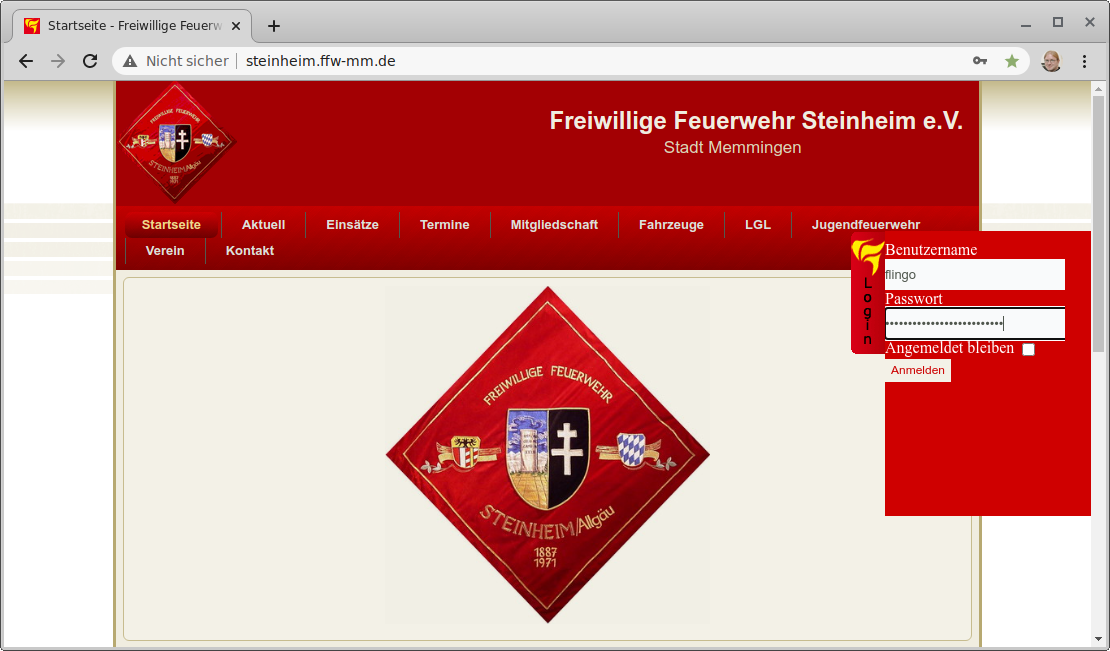
\includegraphics[width=.95\textwidth]{webseite_steinheim.png}
	}
	\only<article>{
	  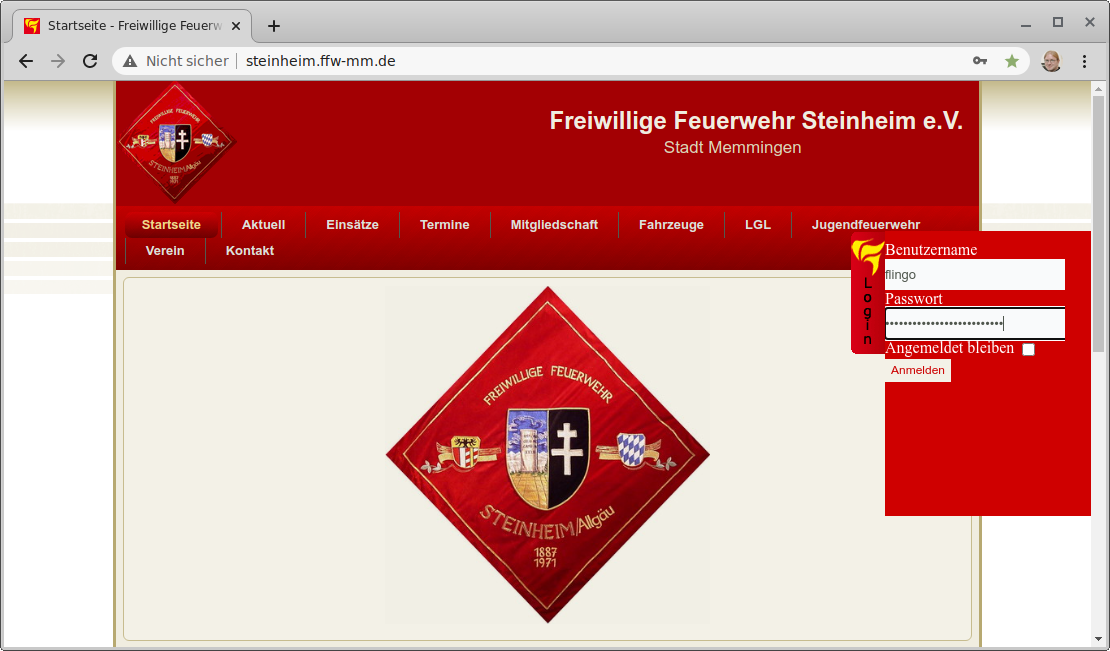
\includegraphics[width=.80\textwidth]{webseite_steinheim.png}
	}
\end{figure}
\end{frame}

\begin{frame}
\only<presentation>{
  \frametitle{Abgreifen Zugangsdaten}
}
\only<article>{
	Das Abgreifen der Zugangsdaten kann beispielsweise über Wireshark erfolgen. Wireshark ist eine Anwendung, die frei im Internet verfügbar ist (\href{https://www.wireshark.org/}{https://www.wireshark.org/}).
}
\begin{figure}[ht]
	\centering
	\only<presentation>{
		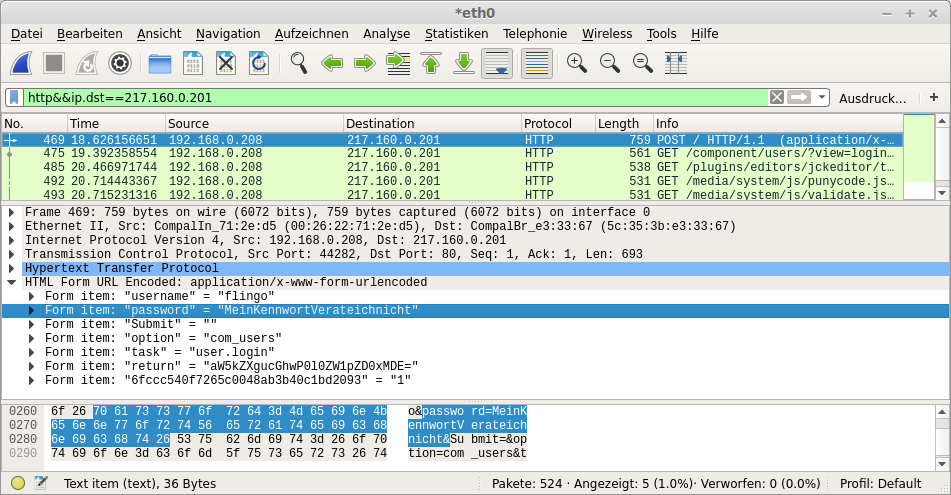
\includegraphics[width=\textwidth]{http_kennwort.png}
	}
	\only<article>{
	  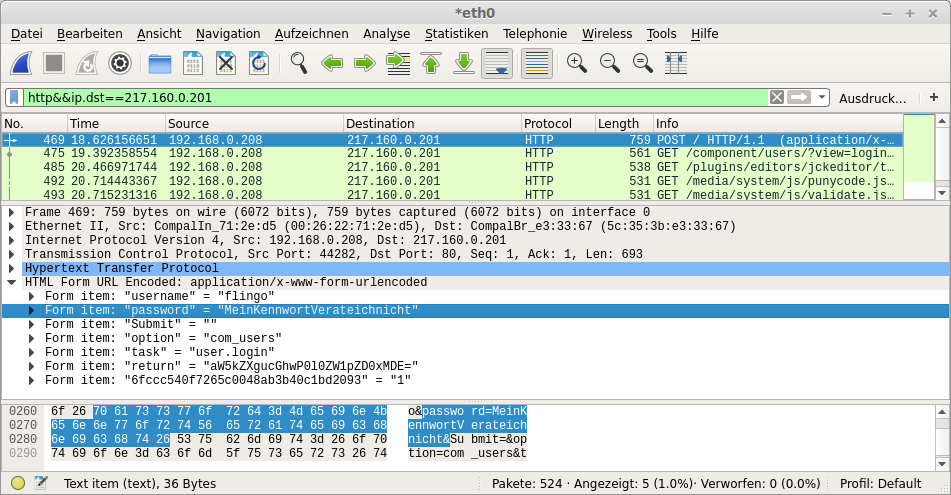
\includegraphics[width=.80\textwidth]{http_kennwort.png}
	}
\end{figure}
\end{frame}

\begin{frame}
\only<presentation>{
  \frametitle{Abgreifen Zugangsdaten}
}
\only<article>{
	Das Programm nslookup erlaubt das Auflösen von Namen zu Internetadressen. Dieses Programm ist auf allen gängigen Betriebssystemen wie Windows, Linux und MacOS verfügbar.
	\newpage
}
\begin{figure}[ht]
	\centering
	\only<presentation>{
		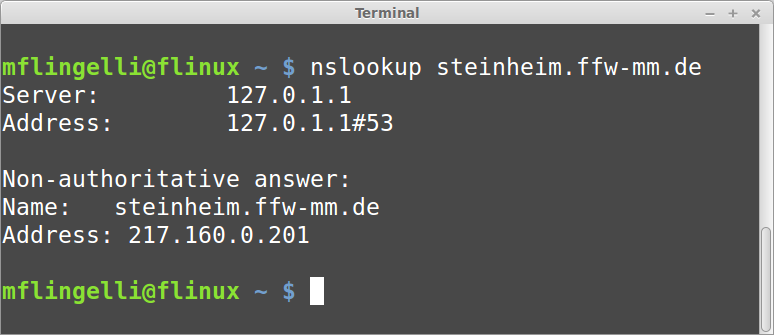
\includegraphics[width=\textwidth]{nslookup_steinheim.png}
	}
	\only<article>{
	  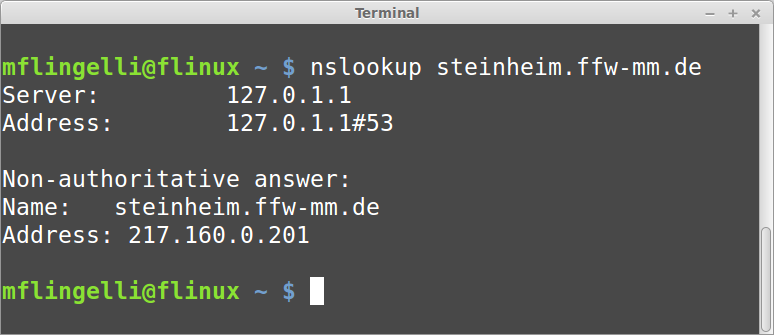
\includegraphics[width=.80\textwidth]{nslookup_steinheim.png}
	}
\end{figure}
\end{frame}

\section{Tipps}

\begin{frame}
\only<presentation>{
	\frametitle{Abschließende Tipps}
}
\begin{enumerate}
	\item Zeit nehmen für den 3-Sekunden E-Mail-Check
	\item Spam-E-Mails direkt löschen
	\item Sicherheitsupdates direkt installieren
	\item Individuelle, sichere Passwörter verwenden
	\item Regelmäßige Back-ups anlegen
\end{enumerate}
\end{frame}

\section{Weiterführende Informationen}

\begin{frame}
\only<presentation>{
	\frametitle{Weiterführende Informationen}
}
\begin{itemize}
	\item BSI für Bürger -- Ins Internet mit Sicherheit:  \href{https://www.bsi-fuer-buerger.de}{https://www.bsi-fuer-buerger.de}
	\item Datenschutzgrundsätze in Deutschland: \href{https://www.datenschutz.org/datenschutzgrundsaetze/}{https://www.datenschutz.org/daten\-schutz\-grund\-saetze/}
	\item Fraunhofer-Institut für sichere Informationstechnologie: \href{https://www.sit.fraunhofer.de/fileadmin/dokumente/sonstiges/Security-Mythen.pdf}{Security Mythen}
	\item Landesfeuerwehrverband Bayern: \href{https://www.lfv-bayern.de/aktuelles/datenschutz-im-verein-und-die-neue-datenschutz-grundverordnung/}{https://www.lfv-bayern.de/aktuelles/datenschutz-im-verein-und-die-neue-datenschutz-grundverordnung/}
\end{itemize}
\end{frame}

\only<presentation>{
\begin{frame}
	\frametitle{Fragen?}
	\begin{figure}[ht]
		\centering
		
\includegraphics[height=.75\textheight]{homer_pythagoras.png}
	\end{figure}
	\scriptsize{Quelle: \href{https://vividkaret.files.wordpress.com/2014/10/homer.png}{\url{https://vividkaret.files.wordpress.com/2014/10/homer.png}}}
\end{frame}
}

\makeatletter
\only<article>{
  \ifthispageodd{
  }{
    \newpage
    \null
  }
  \clearpage
  \newpage
  \thispagestyle{empty}
  \pagecolor{Titelhintergrundfarbe}\afterpage{\nopagecolor}
  \vspace*{175mm}
  \linespread{1.25}
  \begin{flushright}
    \large\textcolor{Titelfarbe}{Ersteller: \@author}\\
    \large\textcolor{Titelfarbe}{Letzte \"Anderung: \@date}\\
    \large\textcolor{Titelfarbe}{\@publishers}
  \end{flushright}
  \linespread{1}
}
\makeatother

\end{document}